\documentclass[10pt,twocolumn,letterpaper]{article}
\usepackage{graphicx}
\usepackage{amsmath}
\usepackage{amssymb}
\usepackage{booktabs}
\usepackage{nicefrac}
\usepackage{algorithm}
\usepackage[algo2e]{algorithm2e} 
\usepackage{multirow}
\usepackage[pagebackref,breaklinks,colorlinks]{hyperref}

% Support for easy cross-referencing
\usepackage[capitalize]{cleveref}
\crefname{section}{Sec.}{Secs.}
\Crefname{section}{Section}{Sections}
\Crefname{table}{Table}{Tables}
\crefname{table}{Tab.}{Tabs.}

\begin{document}
\nocite{*}

\title{Examen}
\author{Emma Fogel}
\maketitle
the front view of a vehicle as input, and outputs a lane edge probability map of the same size as the input image. All the parameters are trained in a completely supervised manner. For each training image, we provide an annotation map where ’1’ indicates this pixel is a positive point laying on the edge of one lane segment, and ’0’ elsewhere.  The en-tire network is end-to-end optimized by stochastic gradient descent.  Note that in every annotation map, the number of positive points are always far smaller than number of negative points. So in the training process, we dynamical weight the loss of positive points and negative points according to their relative amounts, and the loss function is written as:
\begin{equation}
    l_{cls} = \sum_{i}^{B} \sum_{n}^{k} y_{n}^{i} \times \log P_{n}^{i} + \beta(1-y_{n}^{i}) \times \log(1-P_{n}^{i})
\end{equation}
where $B$ is the batch size of one iteration in training process and $P^{i}$ denotes the prediction of the $i$-th sample in this mini-batch.$P_{n}^{i}$ indicating the $n$-th pixel in the image, and $k$ is total  number  of  pixel  in  the  image  which  equals  to $w \times h$. $\beta$ is  the  ratio  of  the  number  of  positive  points  to  the number of negative points, which acts as a dynamic weight for balancing the losses from negative points and positive point. It could be computed by
\begin{equation}
    \beta = \frac{\Sigma y^{i}}{w \times h - \Sigma y^{i}}
\end{equation}
for simplicity.

After training, the network directly produces a lane edge proposal map of the input image where the value of each pixel indicates the confidence of this pixel lies on the edge of one lane segment.
\begin{figure}[H]
    \centering
    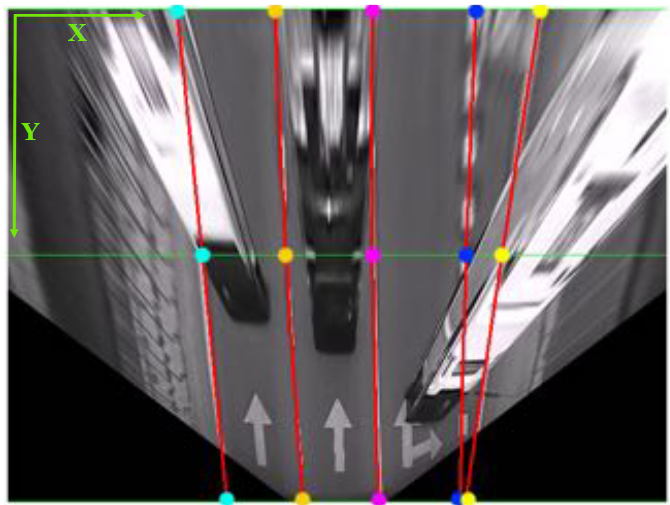
\includegraphics[width=8cm]{images/fig1.png}
    \caption{We present an illustration on how we derive the training objectives of the network. The green line indicates the middle line of the image.  We use three points to locate a lane which is fitted using a quadratic function.}
    \label{fig:Fig3}
\end{figure}
\subsection{Lane line localization network}

In our data, each lane line is represented as a quadratic function, i.e., the shape of each lane is annotated by three continuous numbers. In practice, however, training the net-work to predict the parameters of each quadratic function works poorly as each parameter is usually of significant different  orders  of  magnitude,  e.g.   the  quadratic  term  of  a lane is nearly zero yet the constant term is thousands times larger, which makes the construction of a loss function difficult. Simply normalize the parameters results in disappointing performance as well.  Therefore, we solve the problem by training the network to predict the 
\begin{table}[H]
    \centering
    \begin{tabular}{c|c|c|c|c|c|c}
        \hline \\
         Difficulty & \multicolumn{3}{c}{Easy(1170 lanes)} & \multicolumn{3}{c}{Hard(1035 lanes)} \\
         & Detected & TPR & FPR & Detected & TPR & FPR \\
         \hline\\
         Junhwaet al.\cite{6_} & 916 & 78.2\% & 9.5\% & 801 & 77.4\% & 15.9\% \\
         \textbf{LaneNet} & 1146 & 97.9\% & 2.7\% & 1001 & 96.7\% & 3.9\% \\
         \hline
    \end{tabular}
    \caption{Experiment results.}
    \label{tab:Tab1}
\end{table}
point locations where a lane intersects with the top, middle and the bottom line of an image, respectively.  \cref{fig:Fig3} shows the way we construct the training objectives for each lane.  In our case, the input image has a size of $h \times w$, so the values we train the network to predict are the three $X$ coordination values of the points which lies on the intersections of the lane with three horizontal lines $Y= 0,Y=h/2, $ and $ Y=h$.  We refer these three values to the keys values of a lane. By transferring the training objective from the parameters of a quadratic function to the key values, the predicted values are of relatively similar  orders  of  magnitude  so  that  the  training  becomes stable, and converging at bad local minimum is prevented.A simple matrix multiplication can directly transform the parameters of a quadratic function to the corresponding key values:
\begin{equation}
    \left[K_{1},K_{2},K_{3}\right] = \left[P_{2},P_{1},P_{0}\right]\left[\begin{array}{ccc}
         0 & (h/2)^2 & h^2  \\
         0 & h/2 & h \\
         0 & 0 & 0
    \end{array}\right] ,
\end{equation}
where we use$\left[K_{1},K_{2},K_{3}\right]$to denote the key values of a lane, and$\left[P_{2},P_{1},P_{0}\right]$to indicate the list of quadratic term,linear term and constant term.

While  training  the  lane  line  localization  network  in  a completely supervised way, we can use the average of the $l_{2}$ distance between predicted key values and the real key values of each lane as the loss function and, minimize the distance using stochastic gradient descent. 

Furthermore, using lane edge coordinates as network in-put brings us an additional important benefit.  Considering the large cost of annotating each lane in an image using a quadratic function, and any inaccurate annotations affecting the training result, we design a weakly supervised training method for the lane line localization network, which only requires the number of lanes in a image as ground truth, we call  this  form  of  loss  the  min-distance  loss.   When  using min-distance loss, the loss function is computed by the sum of the distance of each input point to its nearest estimated line.

Specifically,   when  training  the  network  using  min-pervised loss function and additional weakly labelled samples.   Results  are  presented  in  Table  2.   We  can  see  that the weak supervision loss consistently improves the detection on both easy and hard sub-datasets. Further fine tuning the network using weakly labelled data improves the performance on samples with hard difficulties significantly. The fine tuning using weakly labelled data actually enables usto improve the network performance on extreme cases with low  cost.   We  believe  that  more  carefully  collected  hard samples will further improve the network to a even better stage.Additionally, when using a NVIDIA Titan Xp GPU, our lane edge proposal network runs at the speed of 330 frame per second (FPS), and the lane line localization network is even 4 times faster, which enable our entire LaneNet to process images at the speed of 250 FPS. When running on an embedded  GPU  platform,  e.g.   NVIDIA  Jetson  TX1,  the speed turns to 26 FPS without specific modifications, which is fast enough for real-time detection. The model size of the entire LaneNet is restricted to less than 1GB. Both the Com-pact model size and the high running speed further enable the deployment of our LaneNet on vehicles.

\section{Related work}

As a key component of autonomous driving system, lane detection have been widely studied for years.  Despite the intensive demands of real world applications, lane detection remains challenging.  One of the key reasons is the lack of distinct features. To solve this, many works seek to leverage the structural feature of lanes. Vanishing point is considered to be an important feature for the detection of lanes and is used in \cite{9_,16_,19_}.  As for local features, gradient on the lane edges is a popular tool for locating the lanes, e.g.  in[6], two filters which detect left and right edge, respectively,are adopted for finding the strong lane edges in the images.However, gradient based detection methods are vulnerable to scenarios with complex irrelevant objects.  From our observation, the performances of gradient based methods drop dramatically when large amount of other vehicles appear in the images, which are unavoidable in real world scenarios.

In recent years, with the fast development of deep learning and the hardware support, a lot of lane detection methods based on deep neural networks have emerged and show excellent  performances  since  the  training  of  deep  neural network enables detection methods to learn features that are far more robust than the hand-crafted features.  Alexandru Gurghian \textit{et al.} propose DeepLanes which use deep neural network to estimate lane position on the both side of the vehicle.   Jun Li \textit{et al.} use a multitask convolutional neural network to simultaneously detect the presences and the geometric attributes of the lane marks in a patch of the image,  however,  the  patch  based  detection  makes  it  hard  to infer the global structure of the lane lines on the road, thus is incapable of offering decisive information for navigation,so they propose to further combine the convolutional neural networks with recurrent neural networks to introduce context information and make structural predictions. Similar to our method,  Xue  Li \textit{et al.} propose  using  neural  networks to detect the edge of lane lines, and use Hough transform to detect different lanes which the robustness might be weak  when  encountering  with  complicated  scenarios  like extremely curved lane lines.A more comprehensive review on recent advances in lane detection can be found in \cite{13_}.

\section{Conclusion}

In this paper, we proposed a lane detection method consists of two deep neural networks.  The lane edge proposal network takes an IPM image of the front view of a vehicle as input and produces a lane edge proposal map. Given the lane edge map, the lane line localization network is then in charge of inferring the location of each lane in the image.Our lane detection method does not rely on any assumptions and can be applied to various situations.  Using deep neural network endows our method with great robustness and the two stages detection pipeline reduces the computational cost  and  allows  our  lane  line  localization  network  to  be trained in a manner which combines supervised and weekly supervised learning, this remarkably reduces the cost of la-belling  training  data.   Extensive  experiments  demonstrate the speed, accuracy, and robustness of our LaneNet to diverse scenarios.  The future work will focus on introducing lane tracking to our LaneNet for a more stable video based lane line detection method.

{\small
\bibliographystyle{IEEEtran}
\bibliography{references}
}

\end{document}

